%In this section, the layer is described in terms of the hardware and software design. Specific implementation details, such as hardware components, programming languages, software dependencies, operating systems, etc. should be discussed. Any unnecessary items can be ommitted (for example, a pure software module without any specific hardware should not include a hardware subsection). The organization, titles, and content of the sections below can be modified as necessary for the project.
The data controller layer is responsible for getting data about grocery items including data about prices, stock and store location from different stores then transfer the data to the Shopping Manager subsystem in the Server/Back-end layer. There is one subsystem in the data controller layer, the API manager. Since many stores do not allow web scraping, the developer team decided to use public APIs from stores to gather grocery data.
%\subsection{Layer Hardware}
%A description of any involved hardware components for the layer. For example, if each subsystem is a software process running on an embedded computer, discuss the specifics of that device here. Do not list a hardware component that only exists at the subsystem level (include it in the following sections).

\subsection{Layer Operating System}
Data collector layer get the data from the store public web APIs.
\subsection{Layer Software Dependencies}
A description of any software dependencies (libraries, frameworks, etc) required by the layer.

\subsection{API Manager}
%Descibe at a high level the purpose and basic design of this subsystem. Is it a piece of hardware, a class, a web service, or something else? Note that each of the subsystem items below are meant to be specific to that subystem and not a repeat of anything discussed above for the overall layer.
The API manager is a core component of the data collector. The API manager provides one central point for data collection through web APIs across  different stores.

\begin{figure}[h!]
	\centering
 	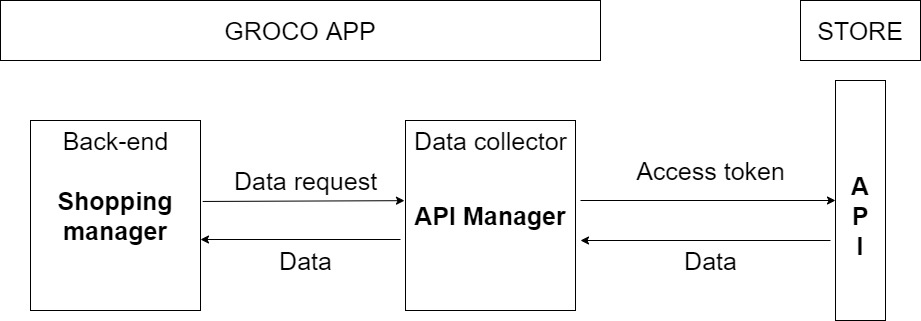
\includegraphics[width=0.80\textwidth]{images/dataCollectorFlowChart.jpg}
 \caption{Data Controller Subsystem}
\end{figure}

\subsubsection{Subsystem Operating System}
Data collector layer get the data from the store public web APIs.

\subsubsection{Subsystem Software Dependencies}
Since many stores do not allow web scraping and do not have public APIs, the development team decide to use Kroger's public web APIs to gether grocery data. 

\subsubsection{Subsystem Programming Languages}
The API manager is written in JavaScript

\subsubsection{Subsystem Data Structures}
%A description of any classes or other data structures that are worth discussing for the subsystem. For example, data being transmitted from a microcontroller to a PC via USB should be first be assembled into packets. What is the structure of the packets?

\subsubsection{Subsystem Data Processing}
%A description of any algorithms or processing strategies that are worth discussing for the subsystem. If you are implementing a well-known algorithm, list it. If it is something unique to this project, discuss it in greater detail.
The API Manager is responsible for storing access tokens to get data from different APIs. The retrieved data will be sent to the Shopping Manager subsystem in the Back-end layer to fulfil the request. The API Manager is also responsible for refreshing the access tokens when they are expired.

